\section{Results}
\label{sec:results}

\subsection{Leakage Current}
\label{subsec:leakagecurrents}

\begin{figure}
	\captionsetup[subfigure]{aboveskip=-1pt,belowskip=-1pt}
	\centering
	\begin{subfigure}[b]{0.49\textwidth}
		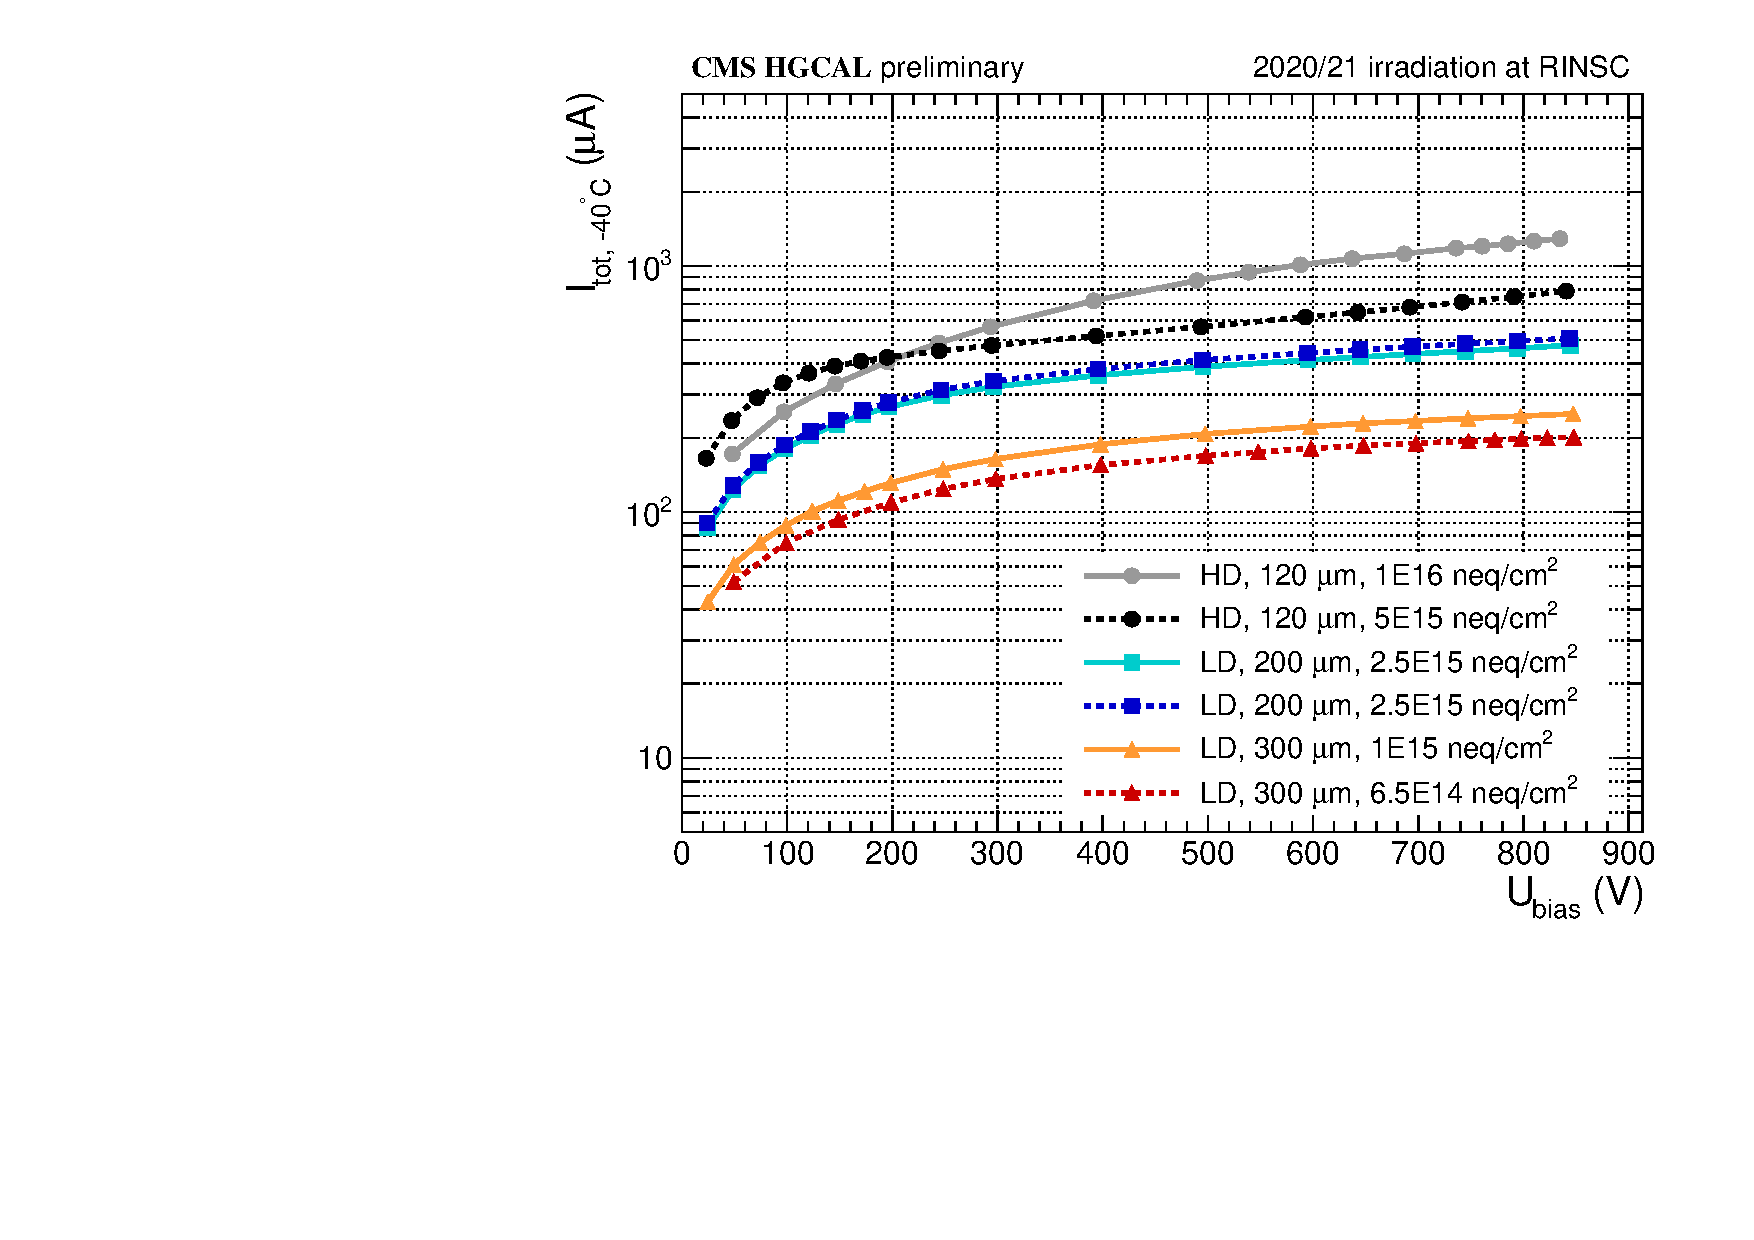
\includegraphics[width=0.999\textwidth]{plots/total_iv/total_current_IV.pdf}
		\subcaption{
		}
		\label{plot:tot_IV_good}
    \end{subfigure}
    \hfill
    \begin{subfigure}[b]{0.49\textwidth}
        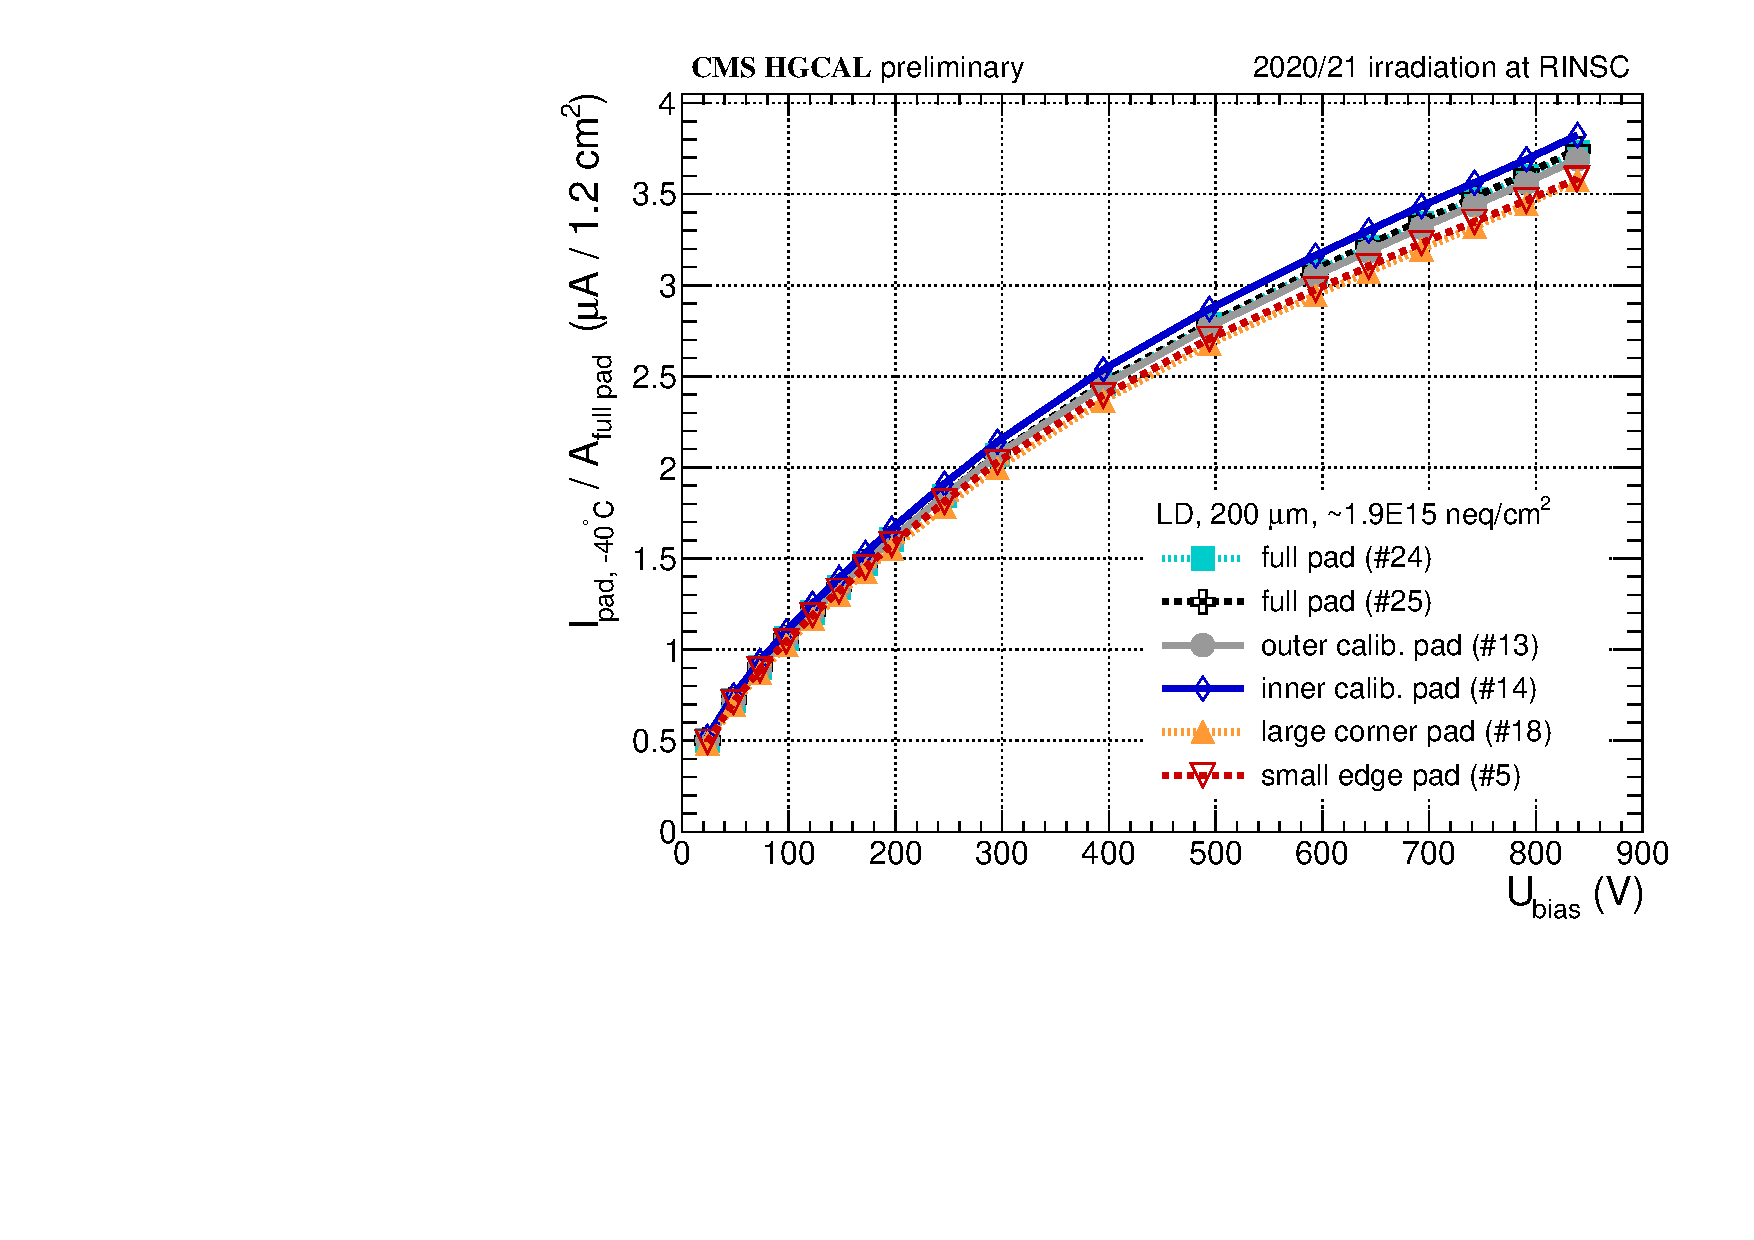
\includegraphics[width=0.999\textwidth]{plots/channel_iv/channel_IV_sensors_channels.pdf}
        \subcaption{
        }
        \label{plot:pad_IV_channels}
    \end{subfigure}

	\caption{
		(a) Two representative full-wafer leakage currents after irradiation (without additional annealing). Measurements were taken at \SI{-40}{\celsius} ($\text{I}_\text{tot, \SI{-40}{\celsius}}$) and for different effective bias voltages ($\text{U}_\text{bias}$). 
        (b) Per-pad leakage currents as a function of the effective bias voltage for different pads with different geometries on one example sensor normalised to the area of full hexagonal pads.
	}
\end{figure}


\begin{figure}
	\captionsetup[subfigure]{aboveskip=-1pt,belowskip=-1pt}
	\centering
	\begin{subfigure}[b]{0.49\textwidth}
		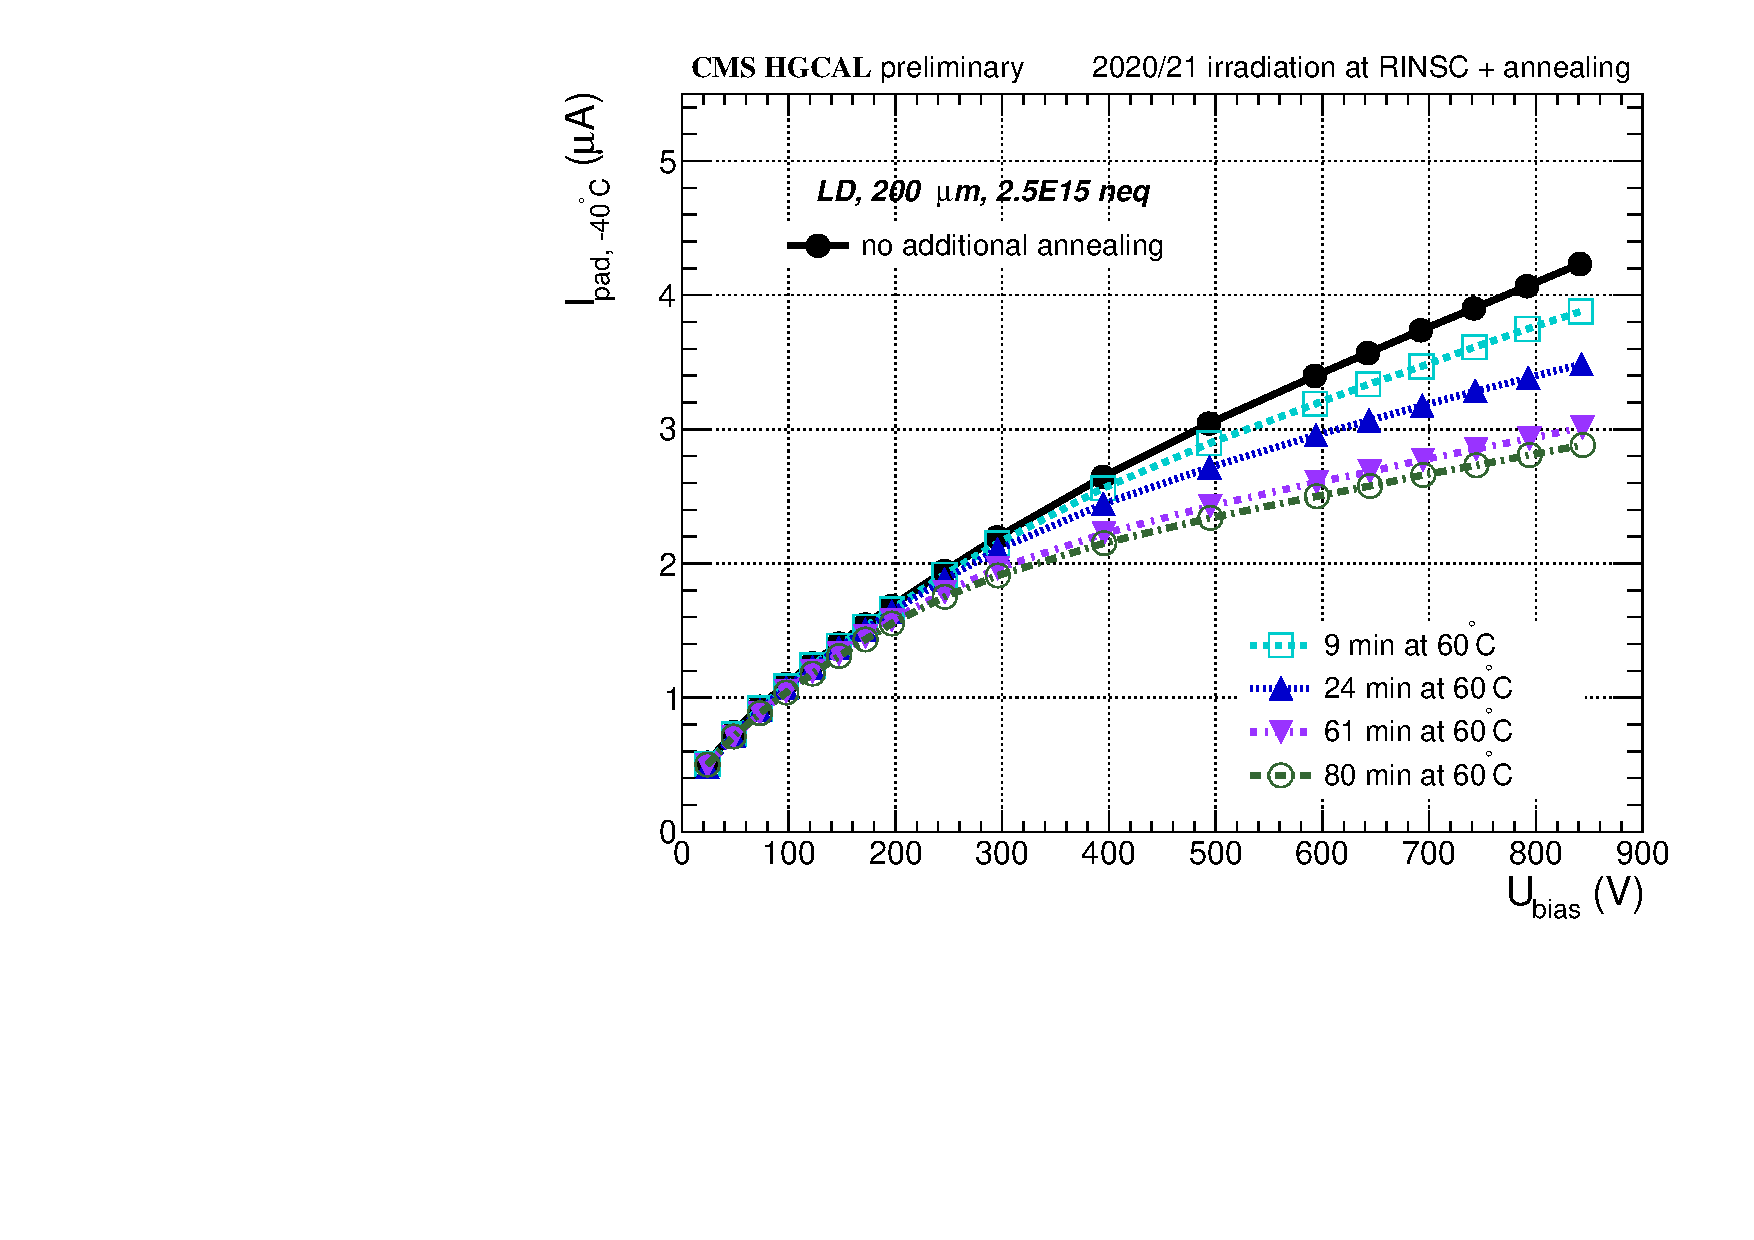
\includegraphics[width=0.999\textwidth]{plots/annealing_iv/annealing_IV_ch24.pdf}
		\subcaption{
		}
		\label{plot:annealing_IV}
	\end{subfigure}
	\hfill
	\begin{subfigure}[b]{0.49\textwidth}
		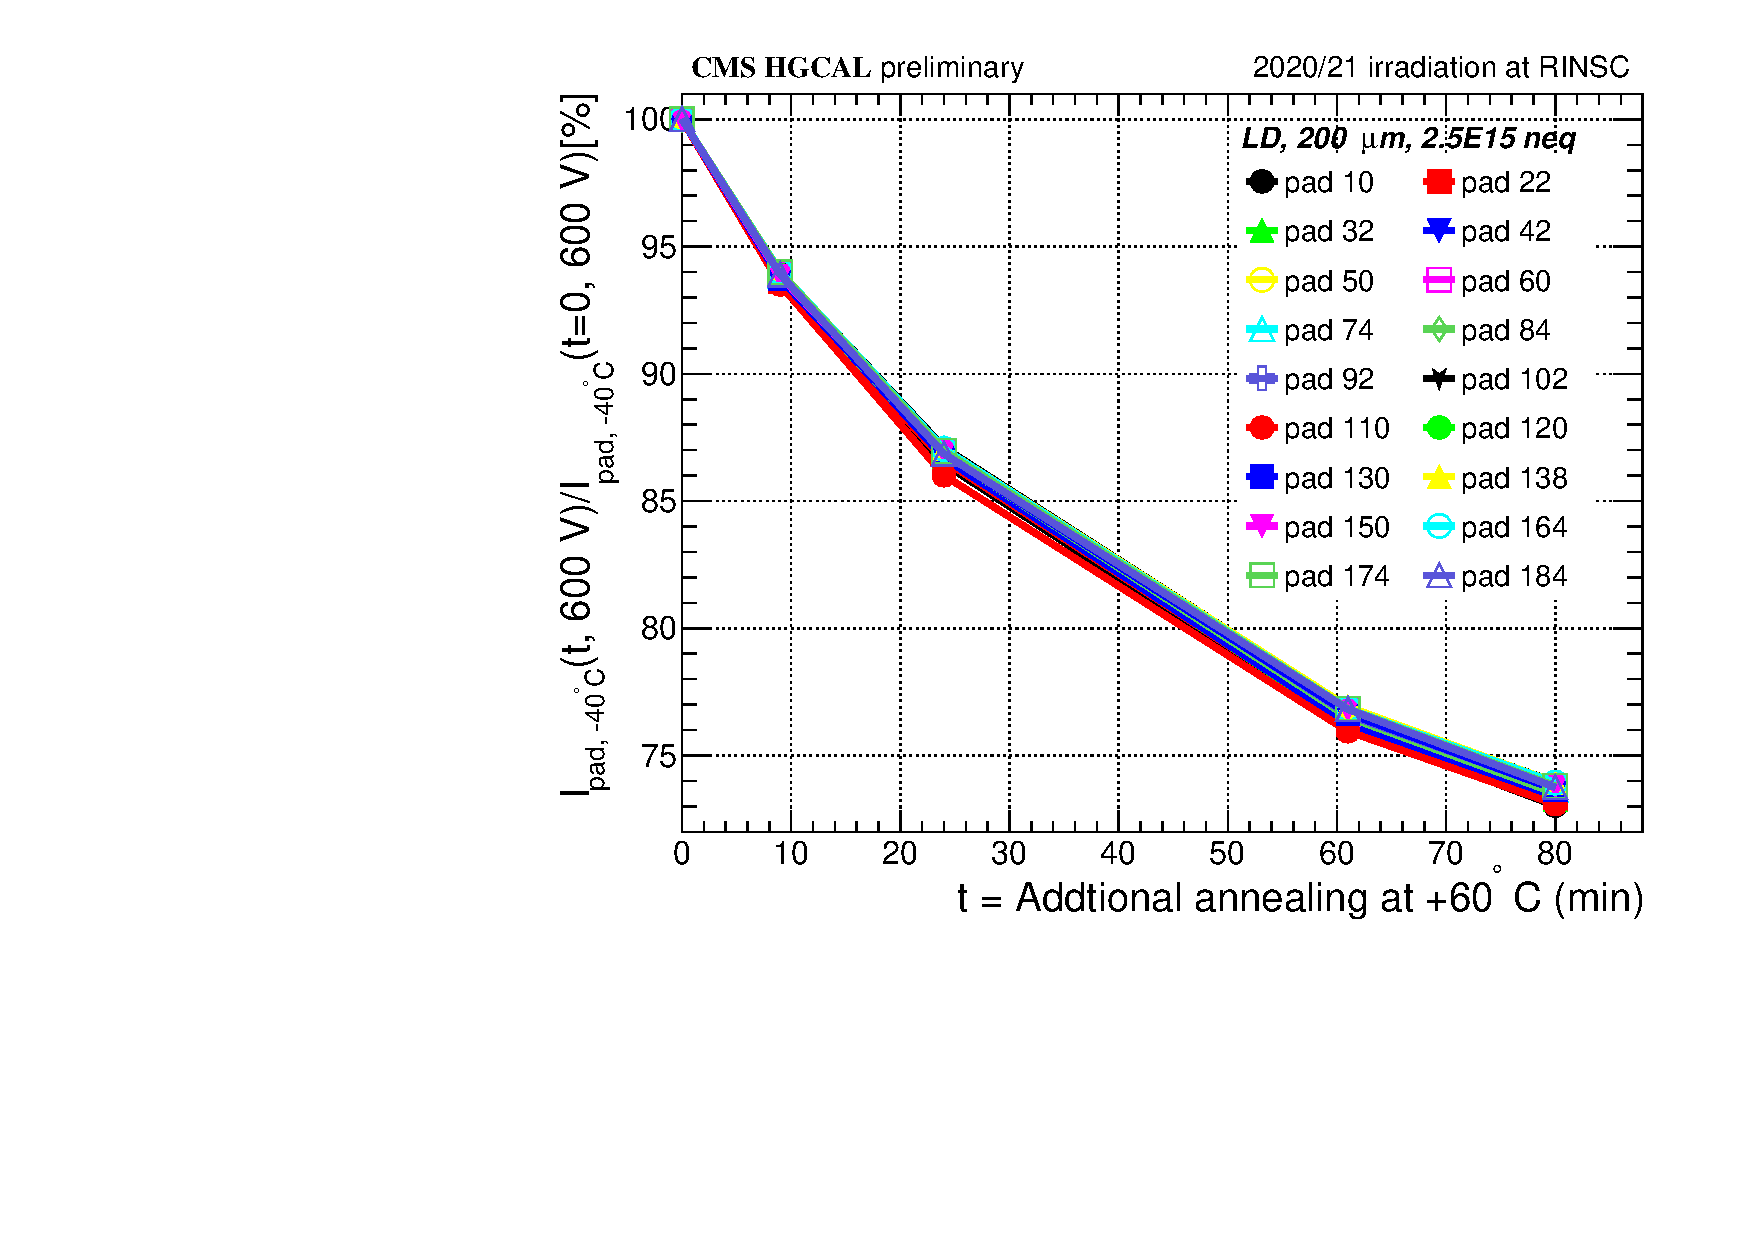
\includegraphics[width=0.999\textwidth]{plots/annealing_iv/annealing_current.pdf}
		\subcaption{
		}
		\label{plot:annealing_current}
	\end{subfigure}    

	\caption{
		(a) IV-curves of a representative full hexagonal pad for different annealing scenarios for a \SI{200}{\micro\metre} low-density prototype sensor irradiated to approximately 2.4$~$E15 1-MeV-neutron equivalents/cm$^{2}$.
        (b) Decrease of the per-pad leakage current (interpolated to $U_\text{bias}=U_\text{dep}$) as a function of the additional annealing time at \SI{60}{\celsius} for a subset of full hexagonal pads.
	}
\end{figure}


\begin{figure}
	\captionsetup[subfigure]{aboveskip=-1pt,belowskip=-1pt}
	\centering
	\begin{subfigure}[b]{0.32\textwidth}
		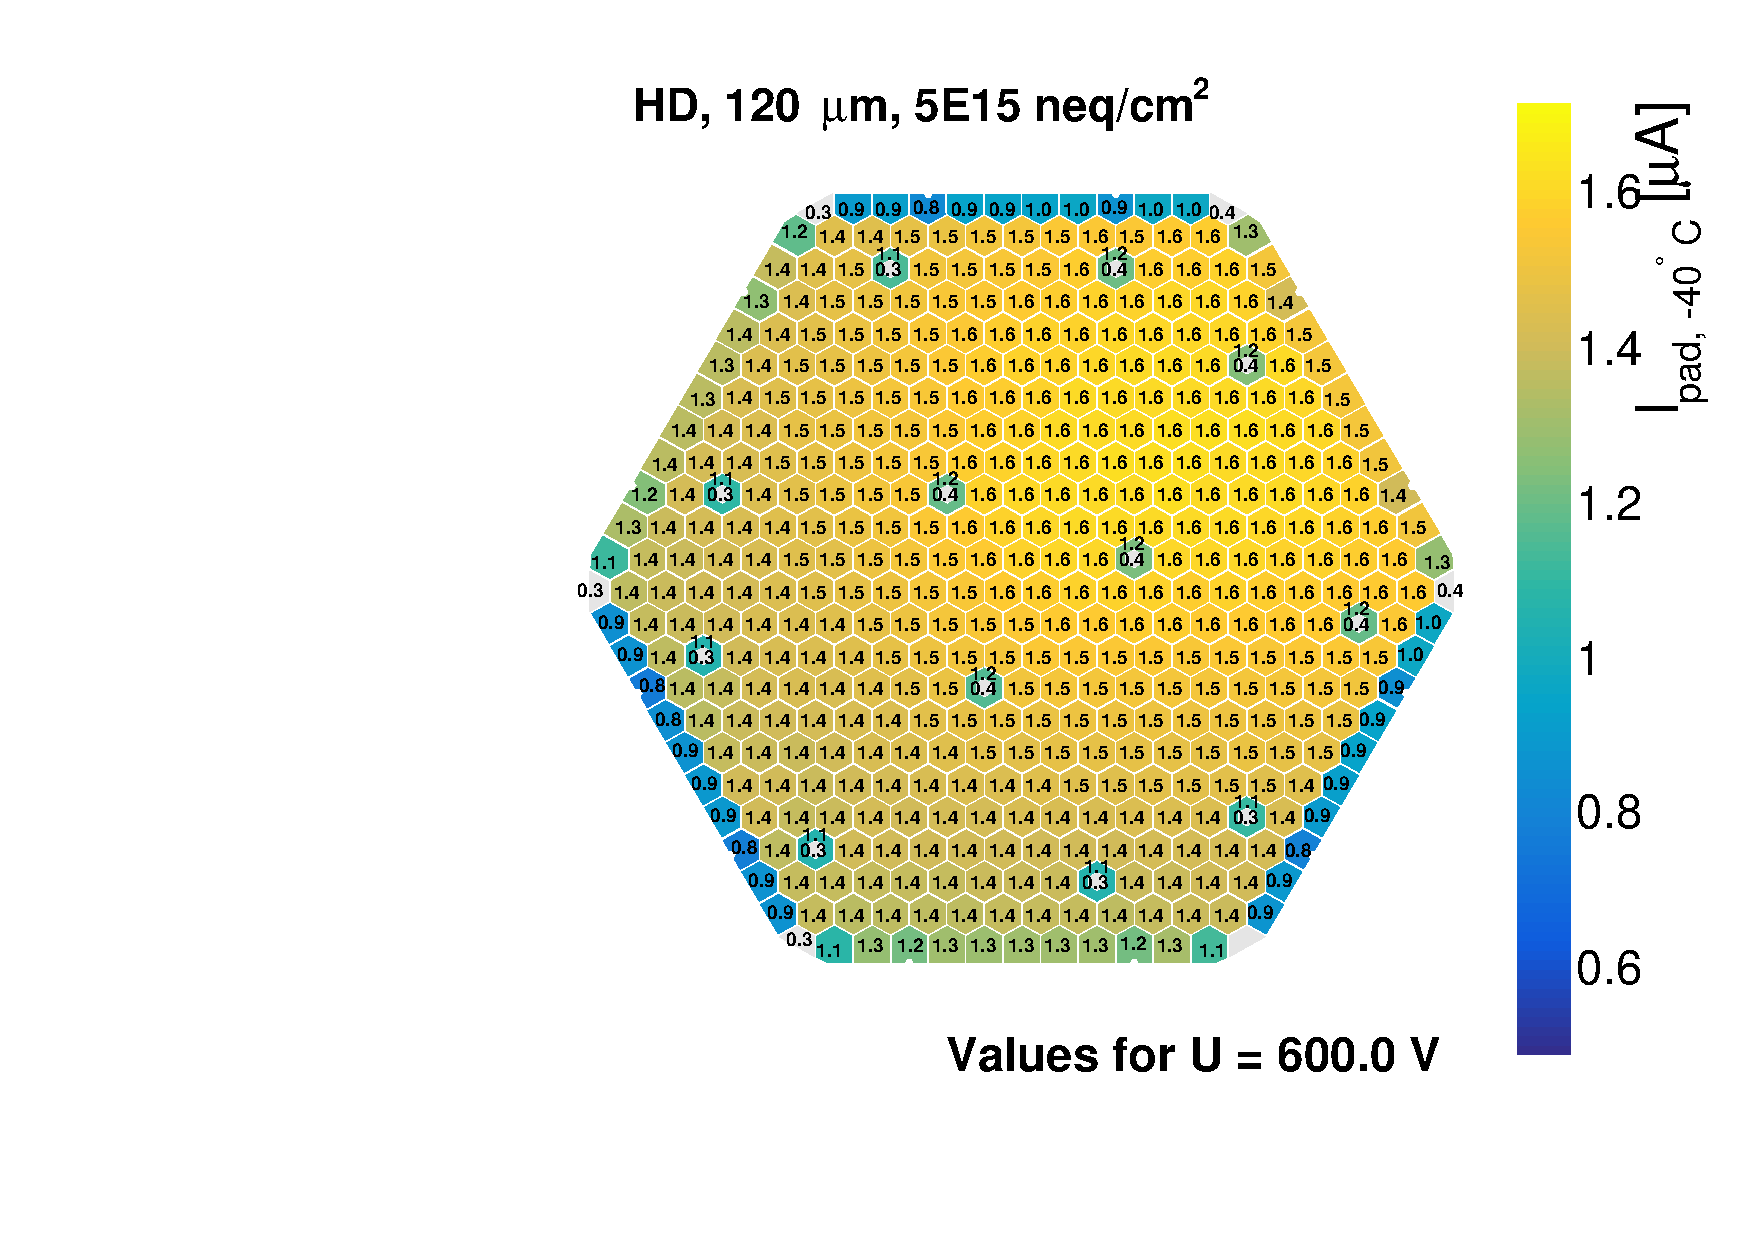
\includegraphics[width=0.999\textwidth]{plots/iv_hexplots/3009.pdf}
		\subcaption{
		}
		\label{plot:iv_hexplot_3009}
	\end{subfigure}
	\hfill
	\begin{subfigure}[b]{0.32\textwidth}
		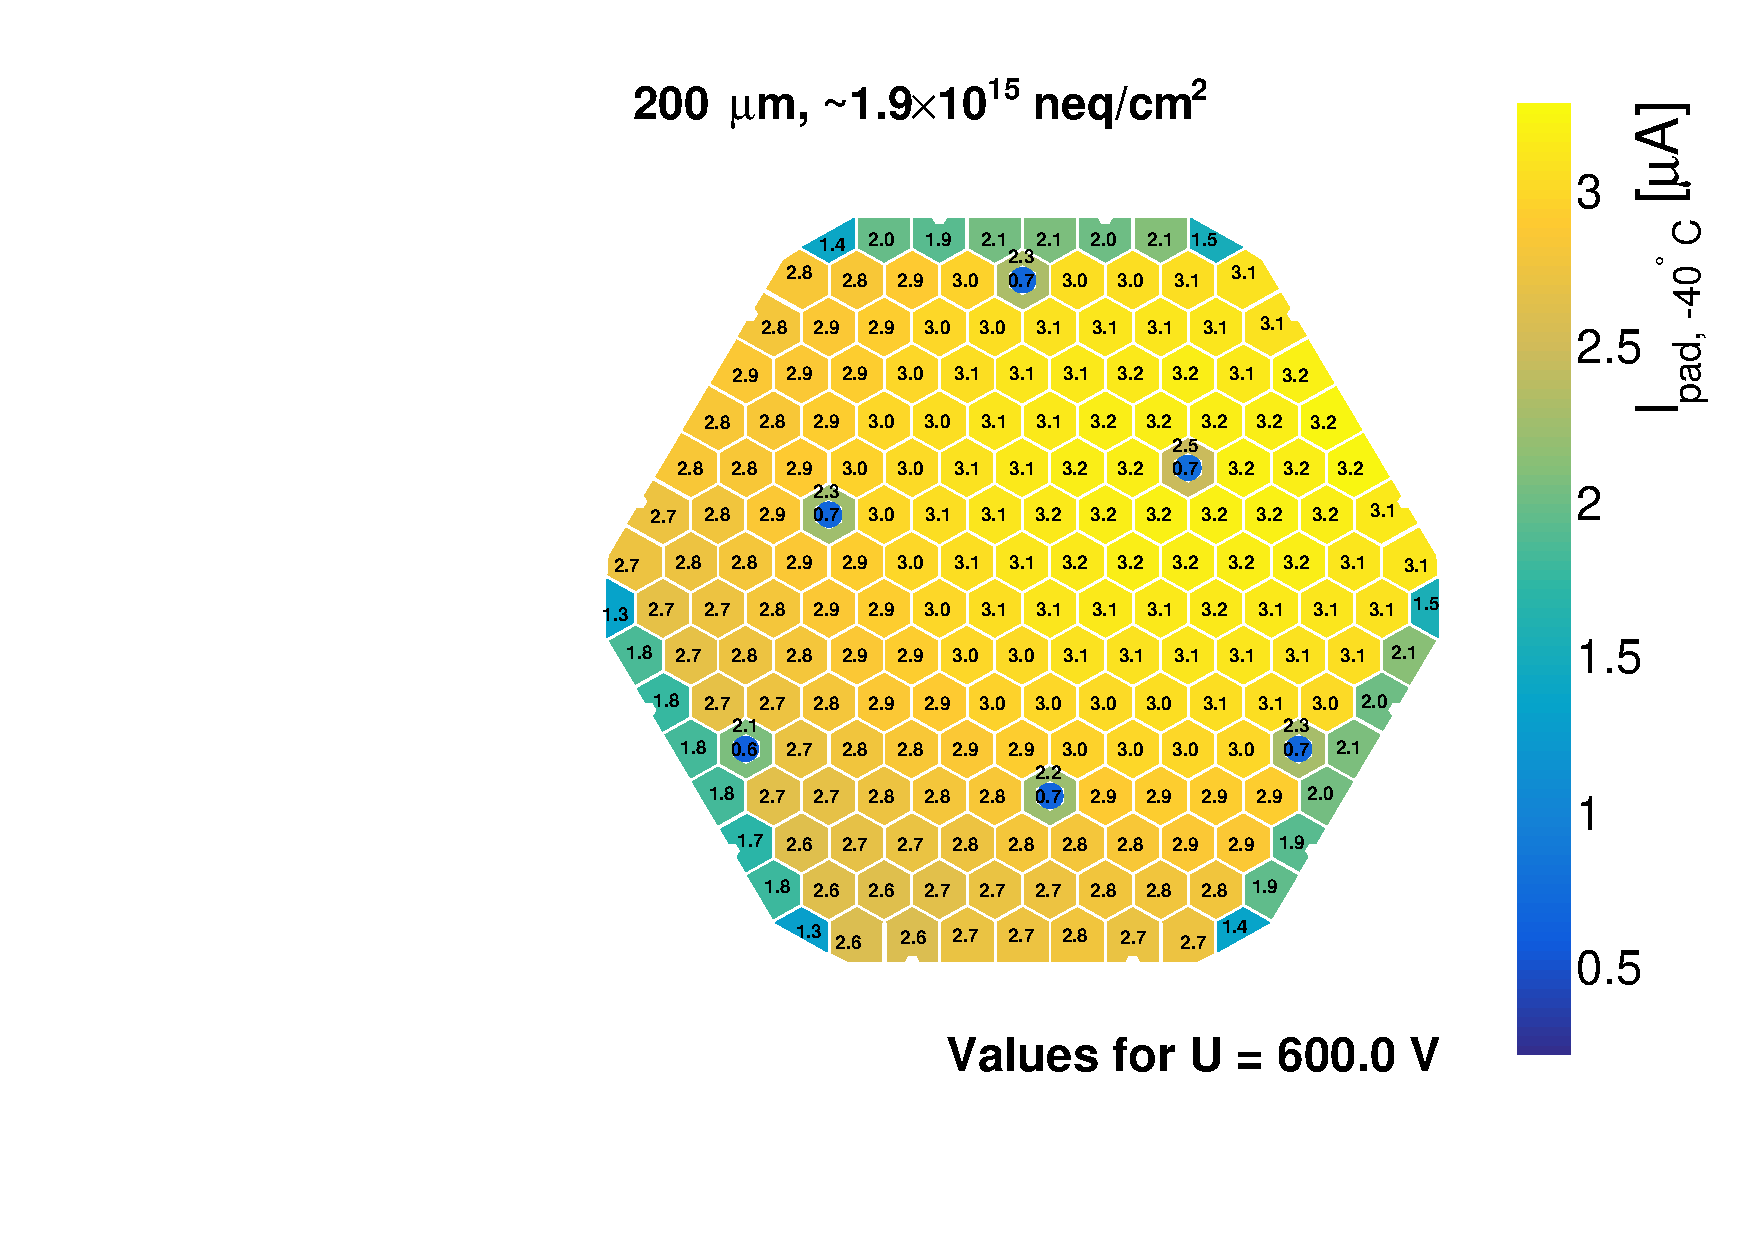
\includegraphics[width=0.999\textwidth]{plots/iv_hexplots/0541_04.pdf}
		\subcaption{
		}
		\label{plot:iv_hexplot_0541_04}
	\end{subfigure}
	\hfill	
	\begin{subfigure}[b]{0.32\textwidth}
		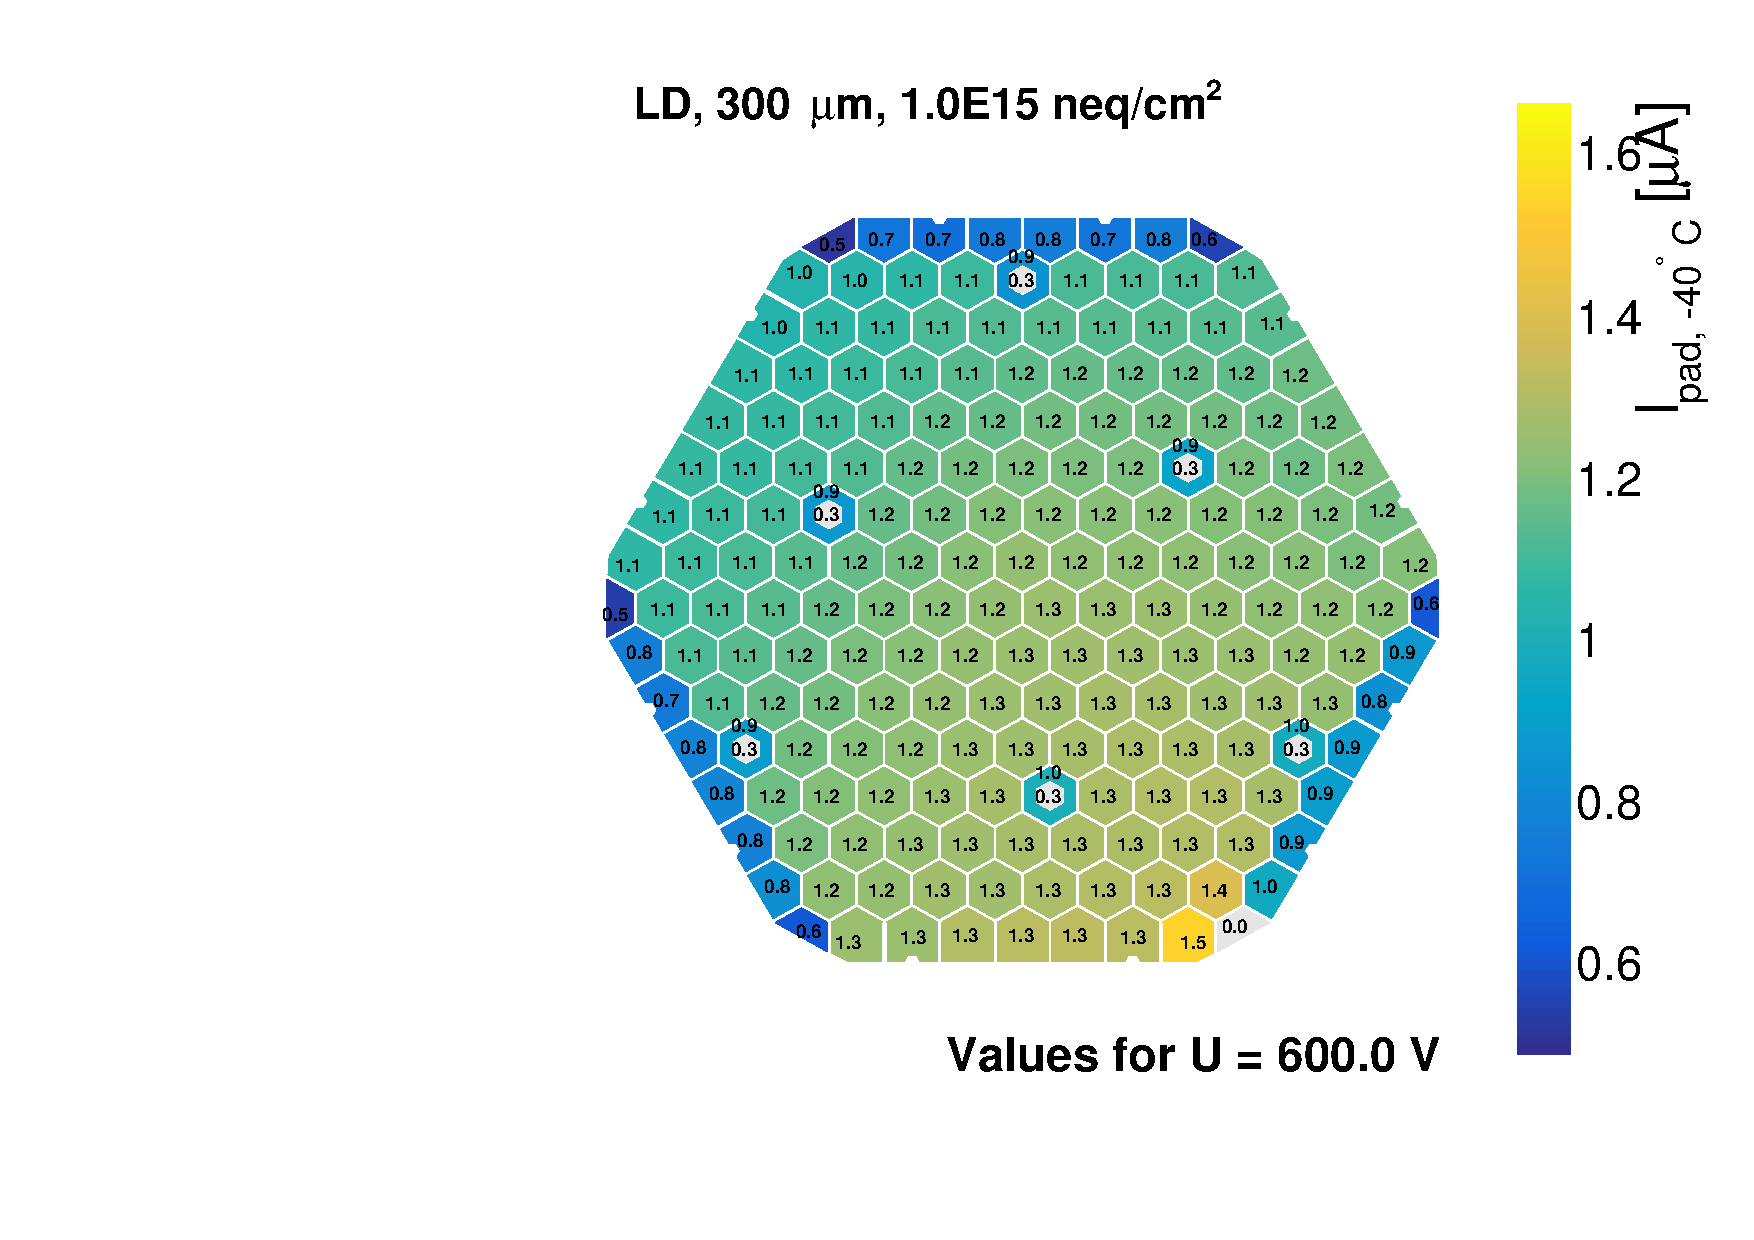
\includegraphics[width=0.999\textwidth]{plots/iv_hexplots/1013.pdf}
		\subcaption{
		}
		\label{plot:iv_hexplot_1013}
	\end{subfigure}
    \hfill
	\begin{subfigure}[b]{0.32\textwidth}
		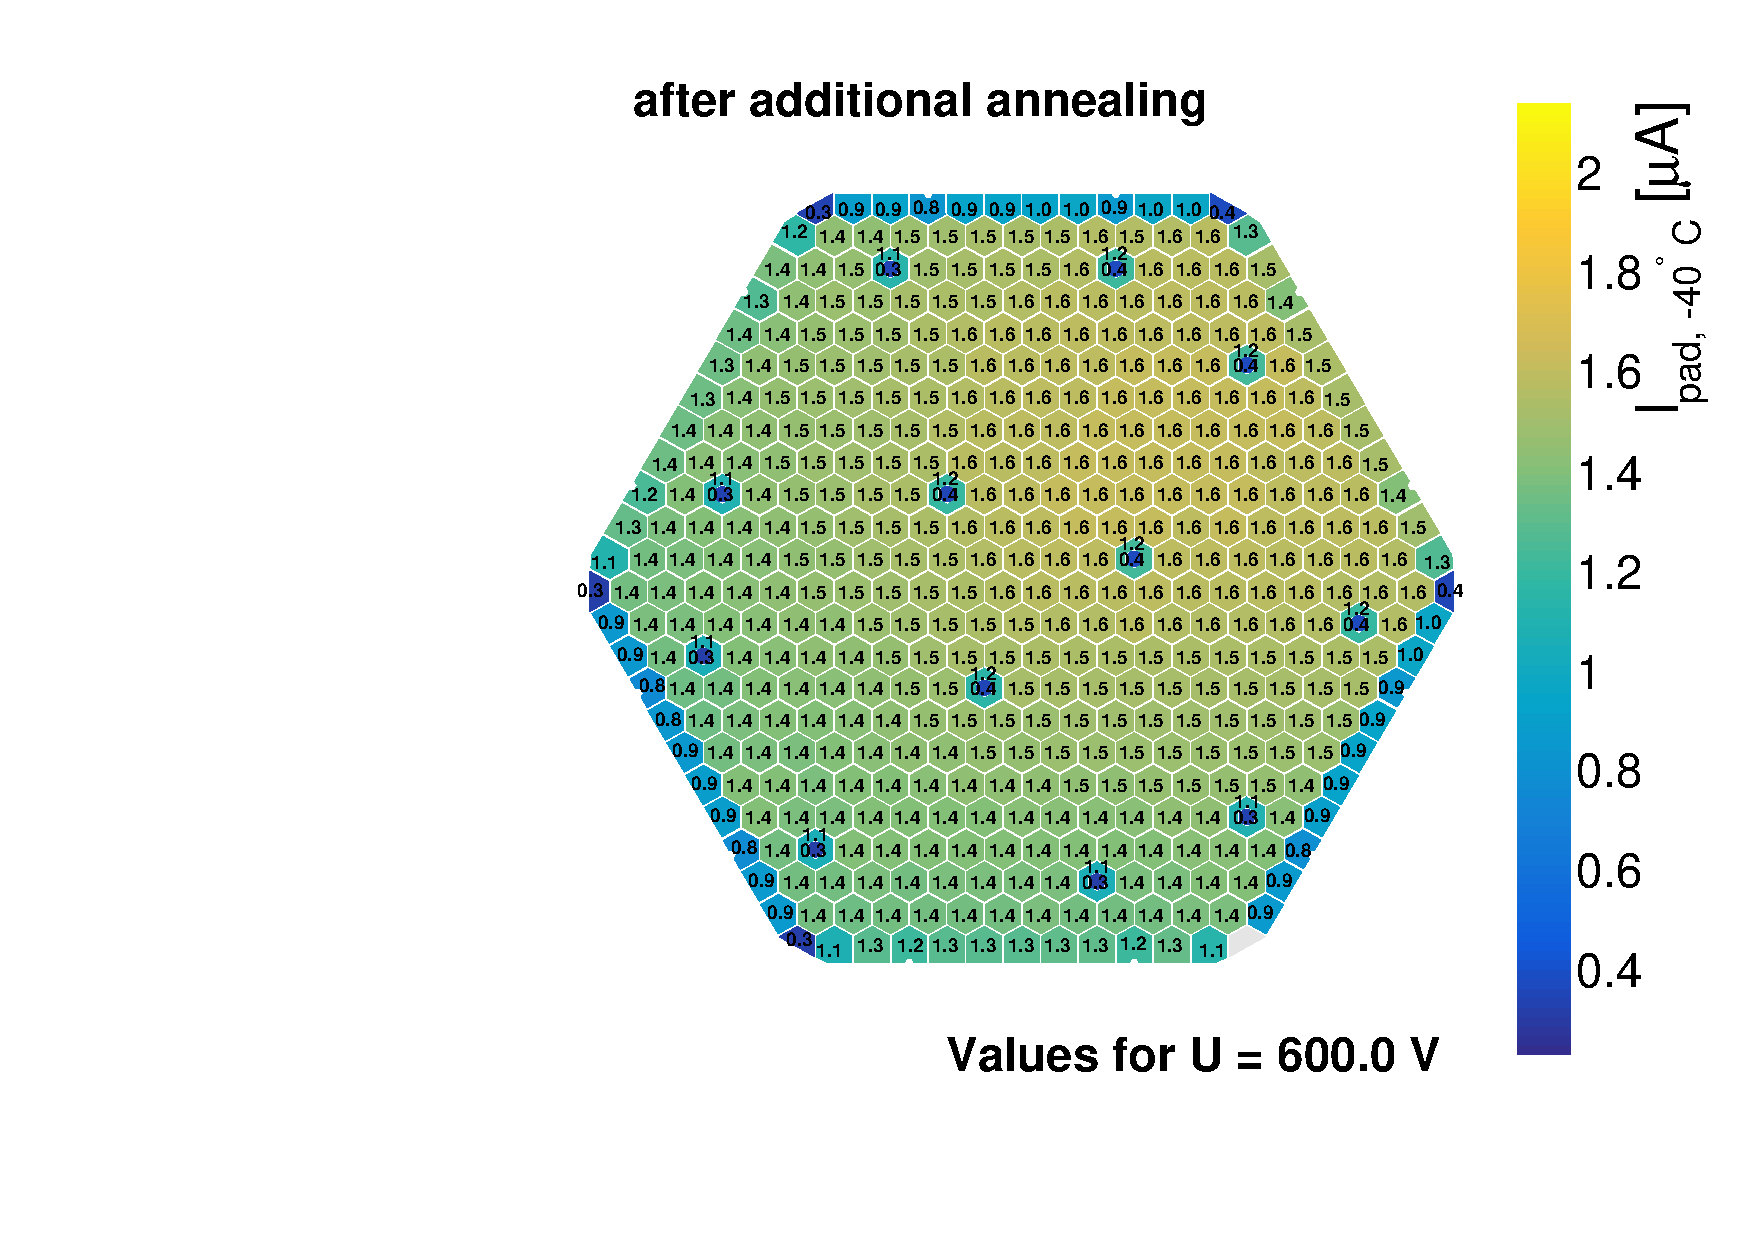
\includegraphics[width=0.999\textwidth]{plots/iv_hexplots/3009_annealed.pdf}
		\subcaption{
		}
		\label{plot:iv_hexplot_3009_annealed}
	\end{subfigure}
	\hfill
	\begin{subfigure}[b]{0.32\textwidth}
		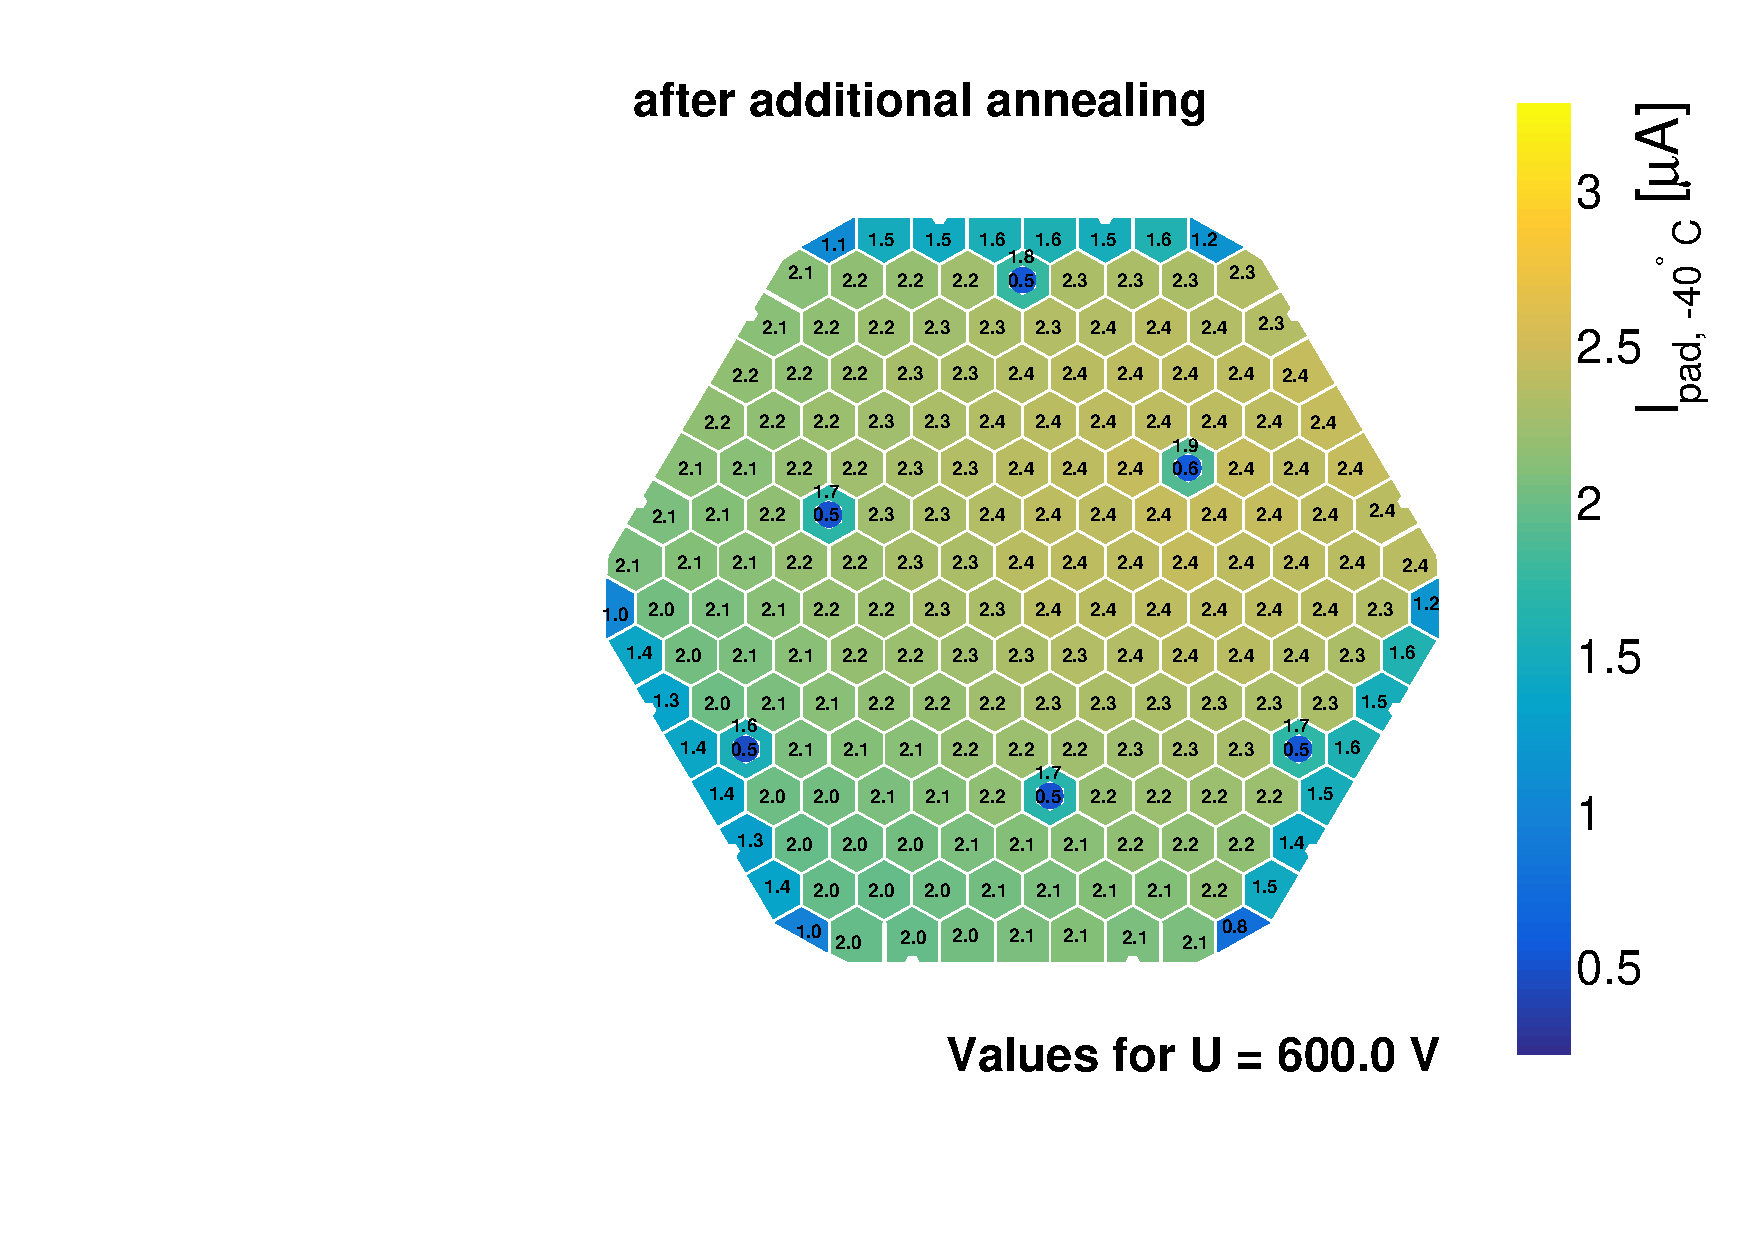
\includegraphics[width=0.999\textwidth]{plots/iv_hexplots/0541_04_annealed.pdf}
		\subcaption{
		}
		\label{plot:iv_hexplot_0541_04_annealed}
	\end{subfigure}
	\hfill	
	\begin{subfigure}[b]{0.32\textwidth}
		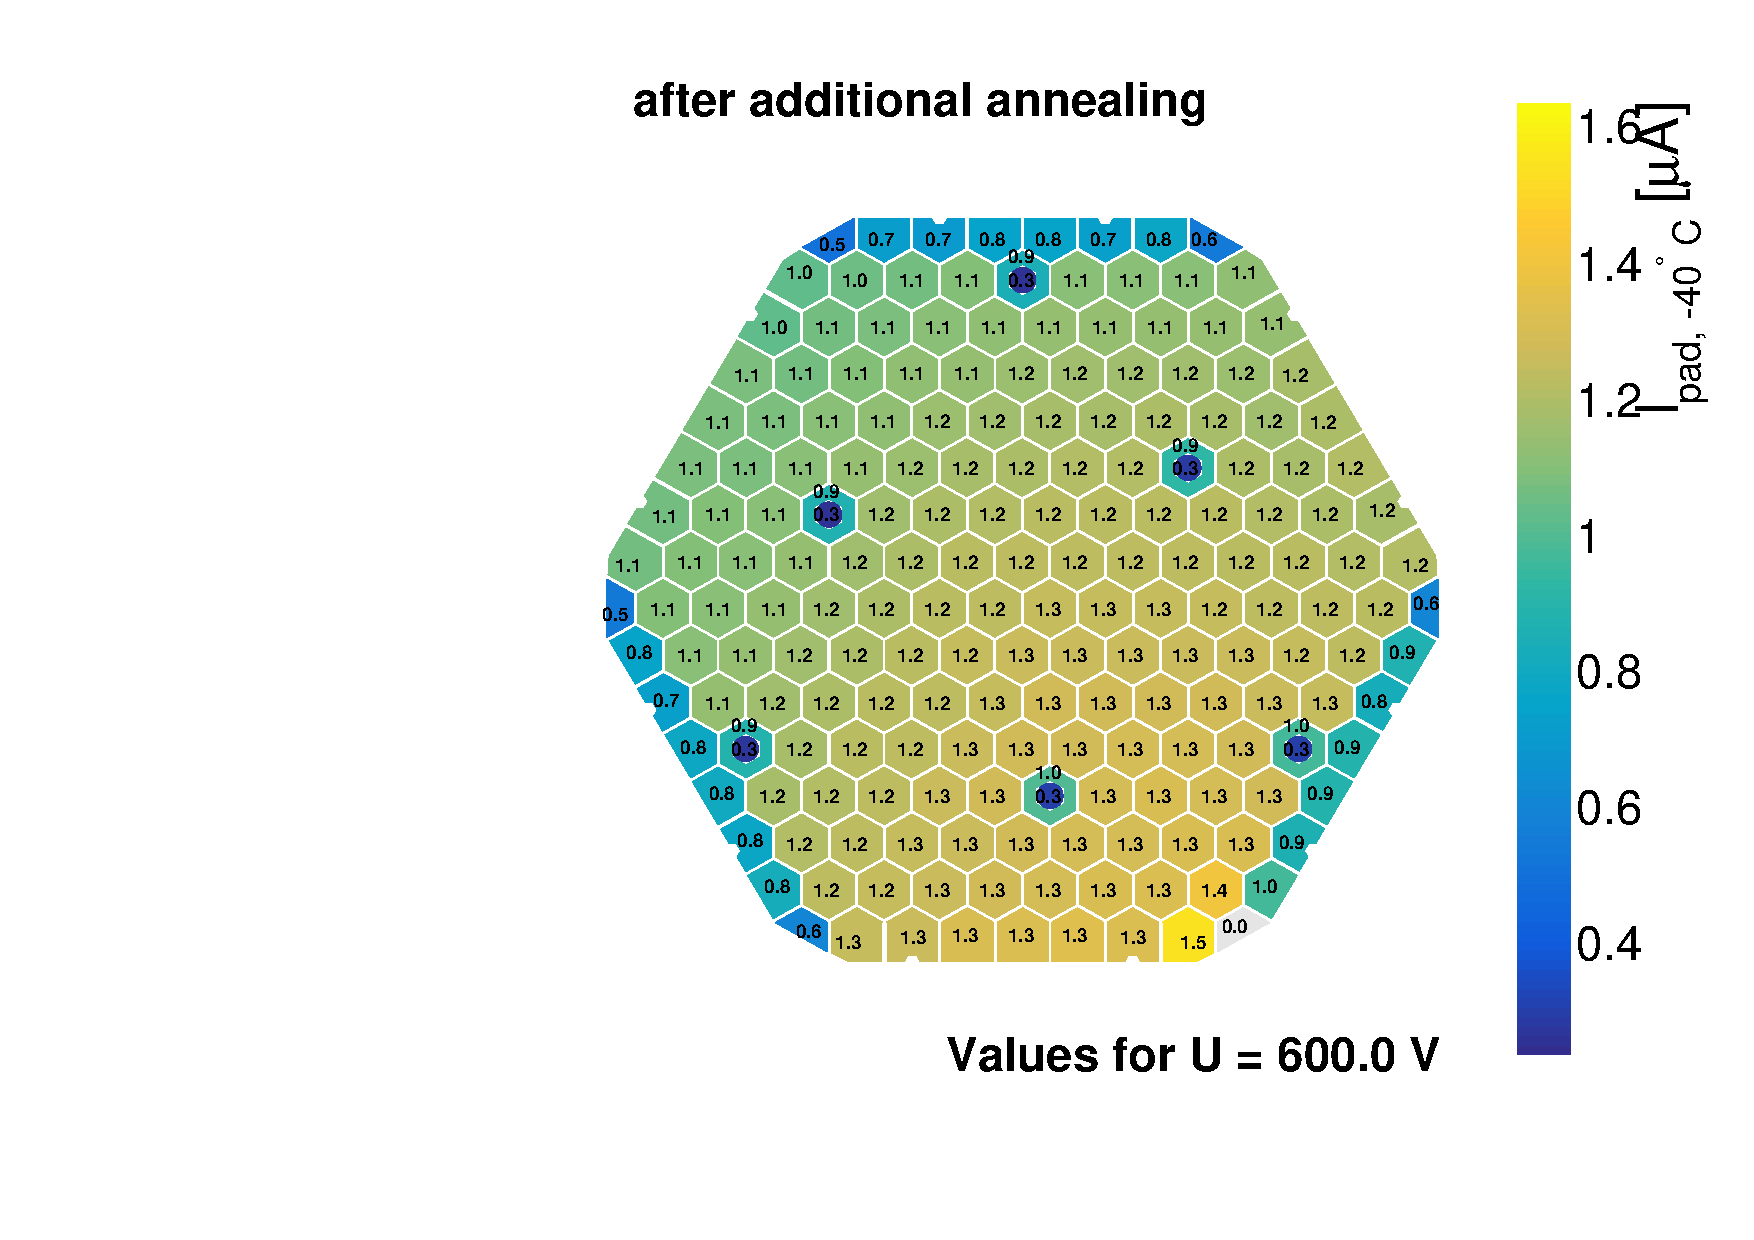
\includegraphics[width=0.999\textwidth]{plots/iv_hexplots/1013_annealed.pdf}
		\subcaption{
		}
		\label{plot:iv_hexplot_1013_annealed}
	\end{subfigure}    
	\label{plot:iv_hexplot}
	\caption{
		Per-pad leakage currents interpolated to an effective bias voltage of \SI{600}{\volt} for three representative sensors from different irradiation rounds before (a-c) and after additional annealing (d-e).
		The chuck temperature profile is corrected for, cf.~\ref{appendix:chuck_temp}.
		Red- or white-colored edge pads correspond to well-understood (however undesired) measurement peculiarities, e.g. unconnected pogo pins.
		Note the different leakage current colour scales.
	}
\end{figure}


\begin{figure}
	\captionsetup[subfigure]{aboveskip=-1pt,belowskip=-1pt}
	\centering
    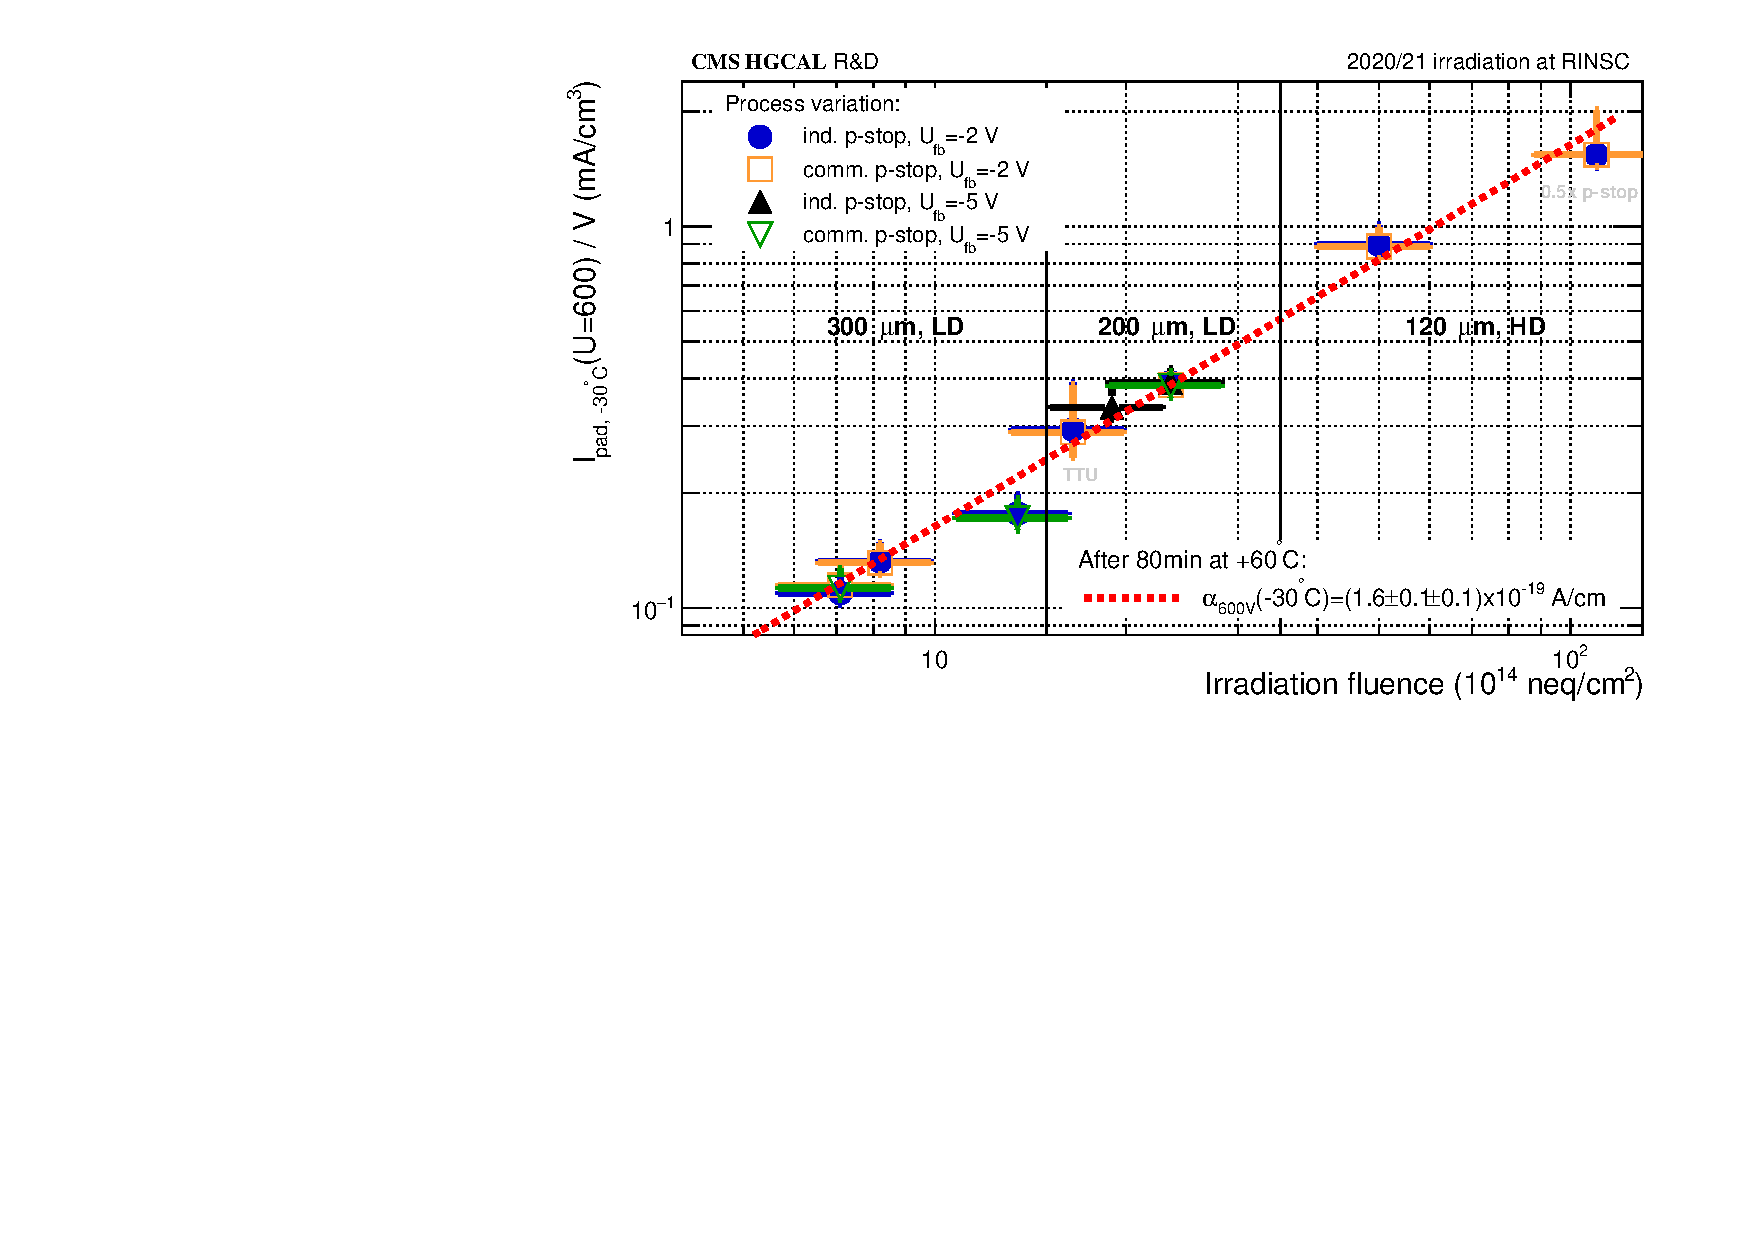
\includegraphics[width=0.69\textwidth]{plots/alpha/alpha_600V.pdf}
    \label{plot:alpha_600}
	\caption{
	    Volume-normalised per-pad leakage current for different fluences at a bias voltage of \SI{600}{\volt}.
        Prototype sensors were characterised after additional annnealing at \SI{60}{\celsius} at CERN and at Texas Tech University (TTU).
		Measured leakage currents are scaled to a room-temperature of \SI{+20}{\celsius}.
        The current-relate damage rate ($\alpha$) is found to be independent of the sensor production parameters investigated in this work.
	}
\end{figure}


\subsection{Capacitance and Depletion Voltage}
\label{subsec:Udep}


\begin{figure}
	\captionsetup[subfigure]{aboveskip=-1pt,belowskip=-1pt}
	\centering

	\begin{subfigure}[b]{0.49\textwidth}
		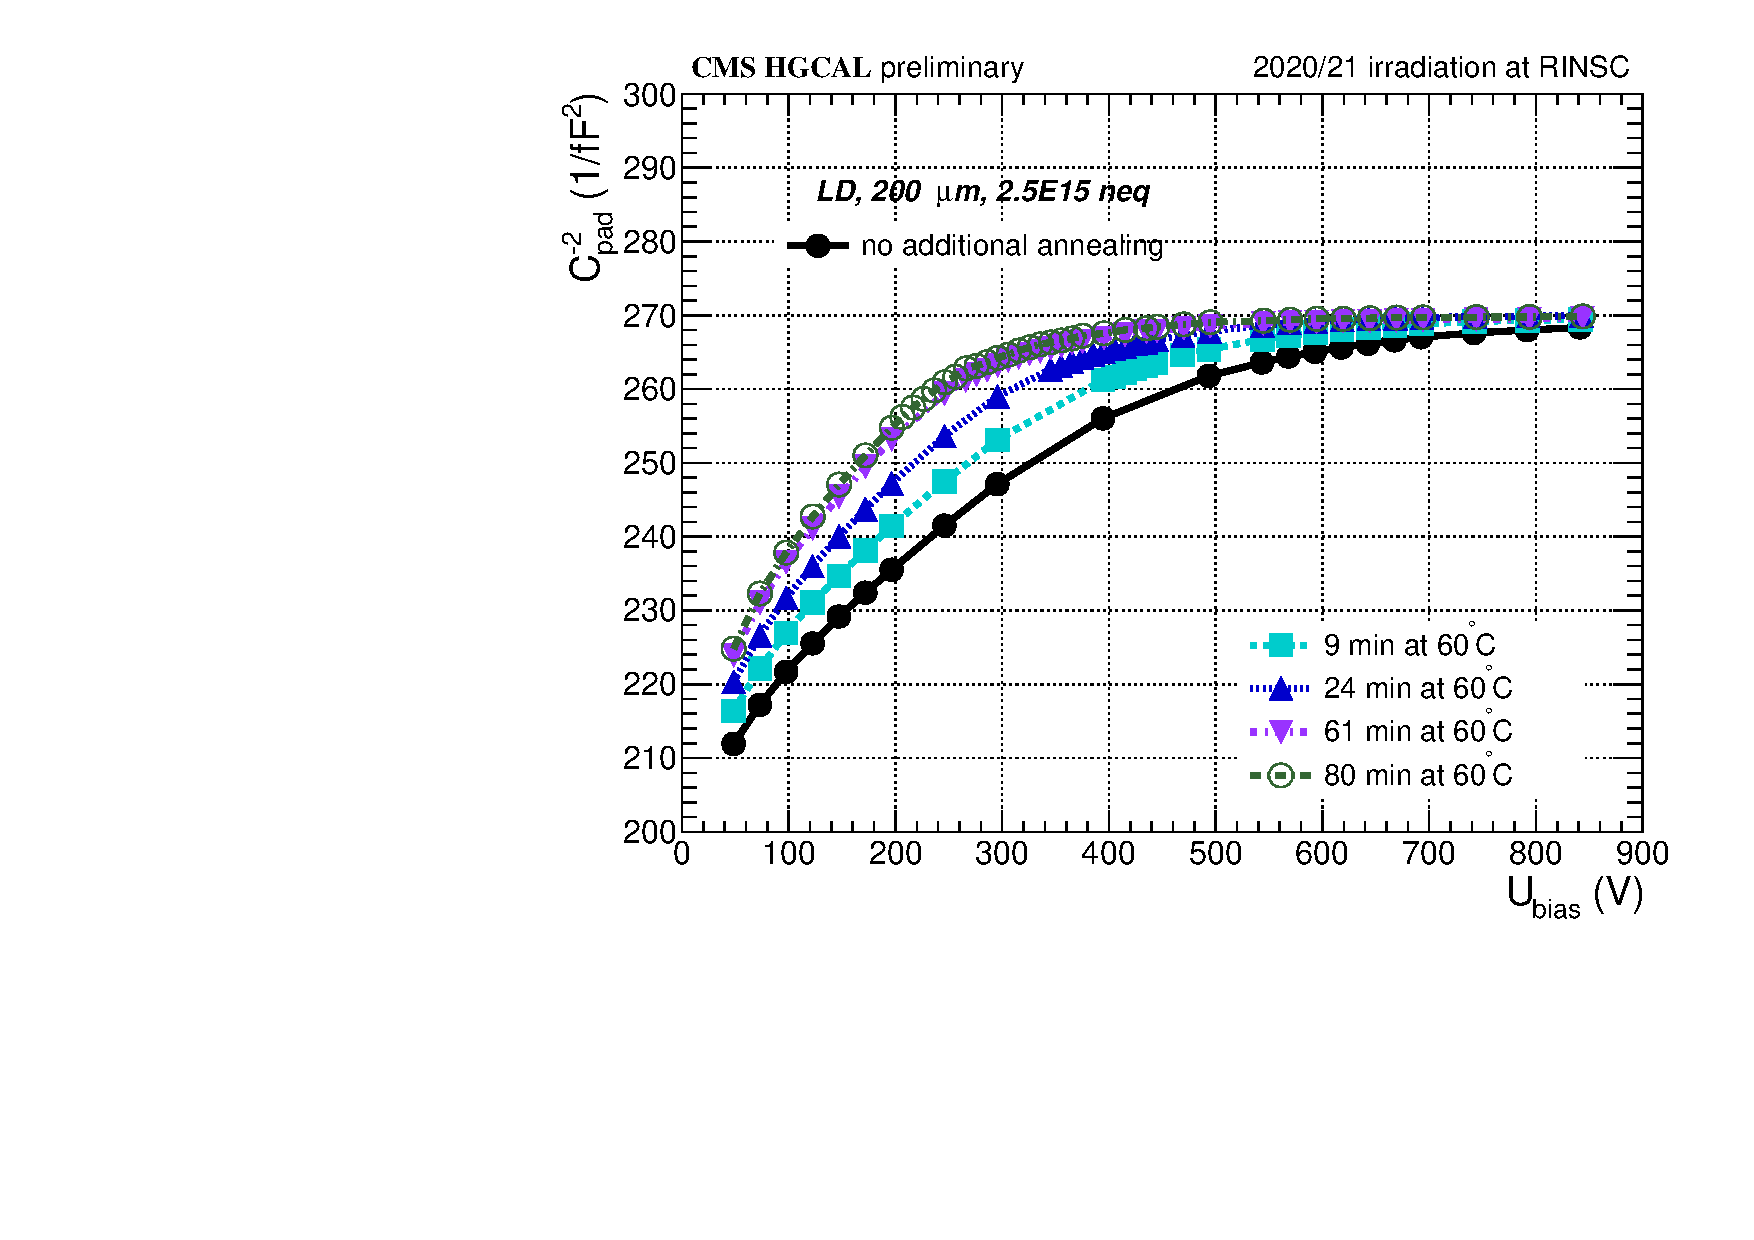
\includegraphics[width=0.999\textwidth]{plots/annealing_Vdep/annealing_CV_ch24.pdf}
		
		\subcaption{
		}
        \label{plot:annealing_CV}
	\end{subfigure}
    \hfill
    \begin{subfigure}[b]{0.49\textwidth}
		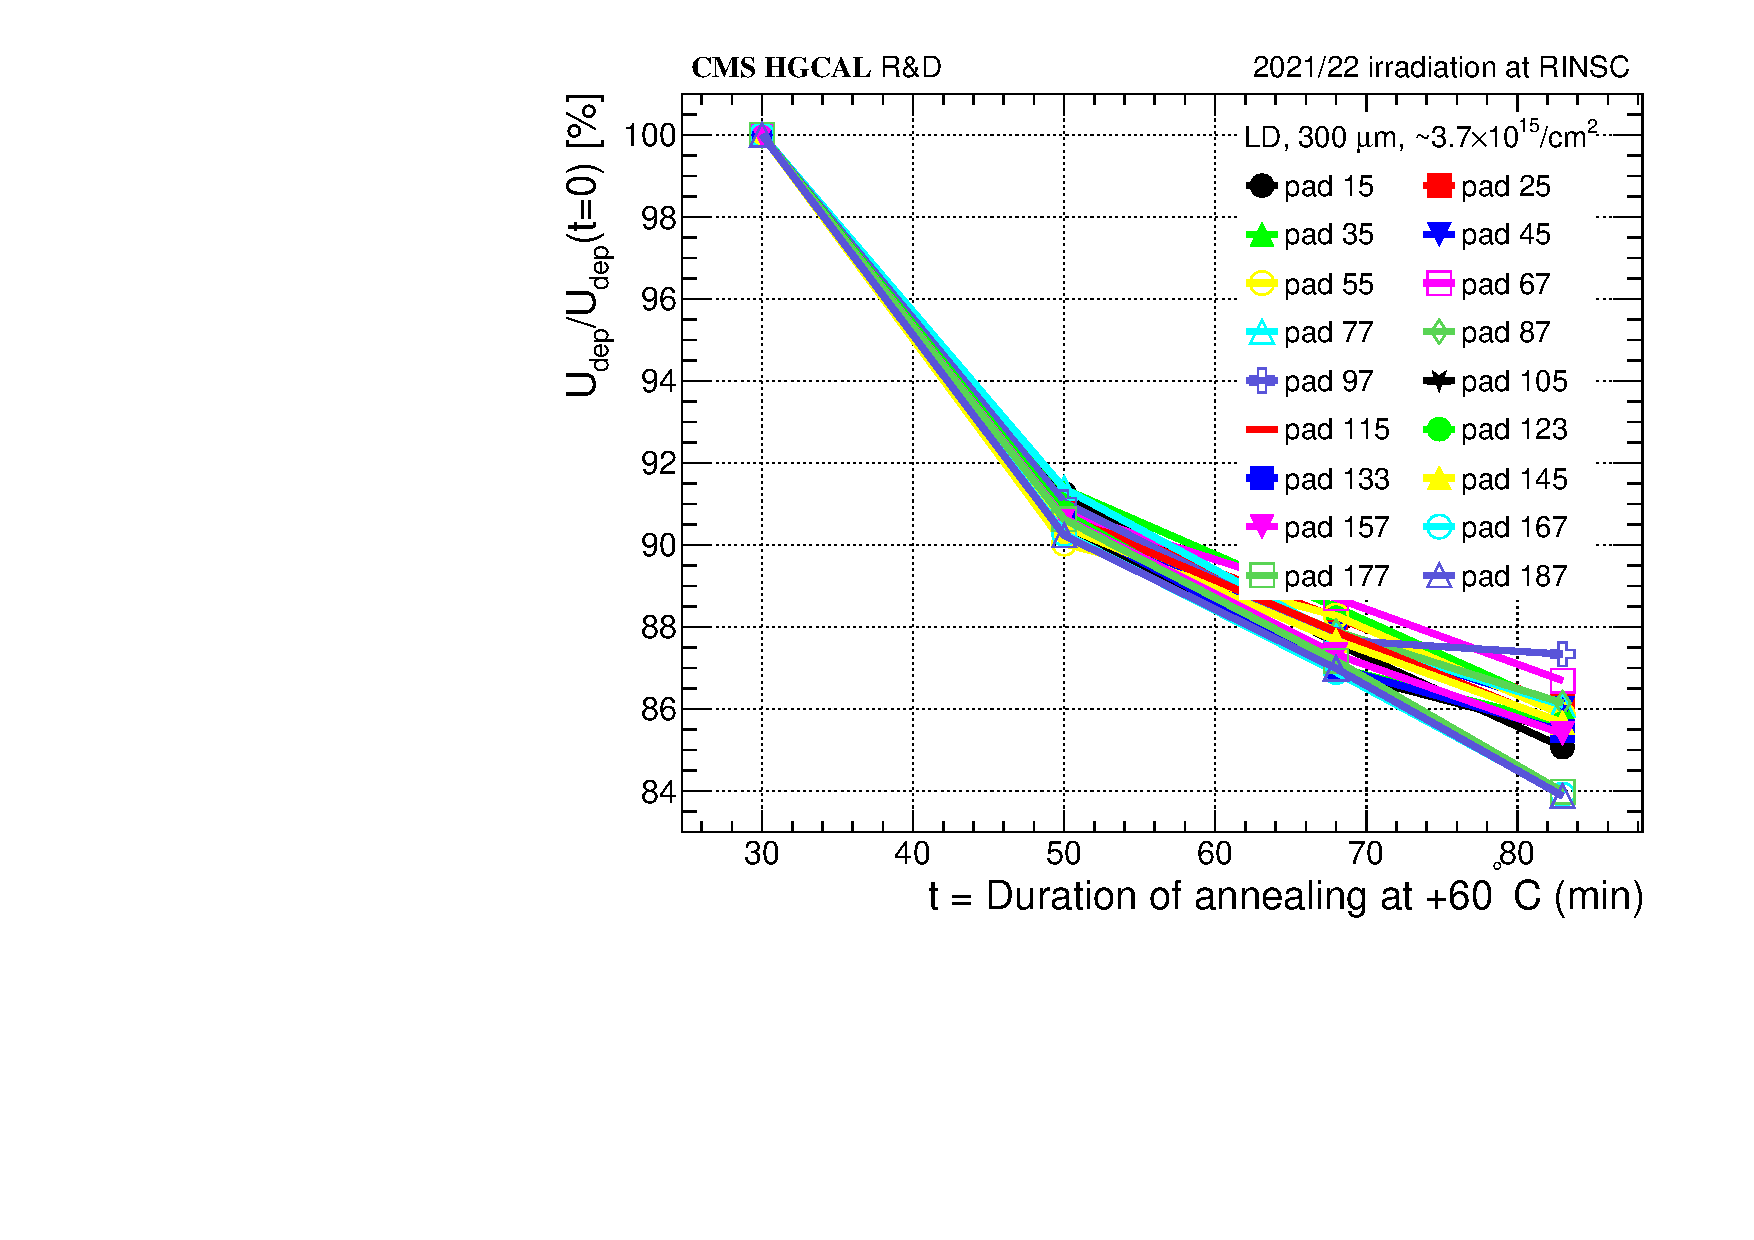
\includegraphics[width=0.999\textwidth]{plots/annealing_Vdep/annealing_Vdep.pdf}
		\subcaption{
		}		
        \label{plot:annealing_Vdep}
	\end{subfigure}
	\caption{
        (a) Inverted CV-curves of a representative full hexagonal pad for different annealing scenarios for a \SI{200}{\micro\metre} low-density prototype sensor irradiated to approximately 2.4$~$E15 1-MeV-neutron equivalents/cm$^{2}$.   
		(b) Relative decrease of the depletion voltage estimate ($U_\text{dep}$) as a function of the additional annealing time at \SI{60}{\celsius} for a subset of full pads.
	}
\end{figure}

%todo: add channels cv, sensors c-2v
%todo: vdep hexplot after annealing, vdep vs fluence